\section{Discussion}
\label{sec:discussion}

The main goal of this chapter was to develop an accurate model for estimating the speed of horses using \gls{imu}. The derived speed from \gls{gps} was used as ground-truth to compare the performances of models trained on five machine learning methods. Each machine learning method was trained on eleven feature sets to compare the estimation accuracy in terms of the number and placement of IMUs on the horse body. The feature sets consisted of time- and frequency-domain features extracted from the output of seven \gls{imu}s, which was an extensive database of acceleration and angular velocity signals.


According to Table \ref{gps_1}, the errors in different speed levels were small enough for practical purposes. The \gls{gps} mean and range of \gls{mape} in measuring slow speed was higher and wider than faster velocities.  The reason is relevant to the accuracy of video footage and the camera, which was the limitation of the current study. The distance measurement accuracy with the recorded video was ±1 cm (approximately the dimension of each pixel, 1 cm × 1 cm), and time duration was always 0.2 s. Therefore, the calculation yielded an accuracy of ±0.05 m/s. This amount of precision in low speed might lead to higher \gls{mape} than faster speeds. This is also true by considering the lower \gls{mae} in 1.5 m/s lower than 4.5 and 7.5 m/s. In total, the errors in none of the speed values were significant, which means this \gls{gps} is accurate in measuring instant velocity in the range of different types of horse gait as same as different speed values \cite{Robilliard187}.


The selected features from the angular velocity signal in limb-related feature sets (Table \ref{tablefeature}) can be explained by the fact that equine limbs move in reciprocating motion. This motion influences the stride frequency, and stride frequency amplifies the locomotion speed. Therefore, a feature extracted from rotation around the z-axis of limb \gls{imu} can be an indicator of change in stride frequency \cite{doi:10.1111/eve.12400,1inproceedings,PMID}. In addition, the sacrum, withers, and poll feature sets had z-axis acceleration signal extracted features as their highest rank features. The explanation can be similar to the limbs since by using vertical acceleration of the mentioned \gls{imu}s, it is possible to determine the periodical pattern of their vertical displacements. Thus, the vertical displacement is affected by the hoof-on and hoof-off rate, i.e., stride frequency \cite{adsd1,456}. 

To analyze the relation of stride frequency and speed in the dataset, hoof-on moments of the right front limb were detected using a validated method from another study \cite{adsd1}. Then, stride frequency was calculated using the timing of detected hoof-ons, time-synchronized with speed values. According to the result shown in Figure \ref{stridevsspeed}, as speed increases, the stride frequency also increases. To investigate the possibility of estimating speed using stride frequency, we fitted second- and third-degree polynomials to the data and computed the accuracy. However, the accuracy was low compared to the results of the machine learning models (2nd-degree polynomial: \gls{mae} = 0.51 m/s, \gls{rmse} = 0.8 m/s and $R^{2}$ = 0.74; 3rd-degree polynomial: \gls{mae} = 0.52 m/s, \gls{rmse} = 1.36 m/s, and $R^{2}$ = 0.73), which is concurrent with the outcome of other studies \cite{articlewalk,trot4.tb04375.x}. Therefore, it requires a more complex model to estimate speed accurately, which has been done successfully in this study.

\begin{figure}[htbp]
\centering
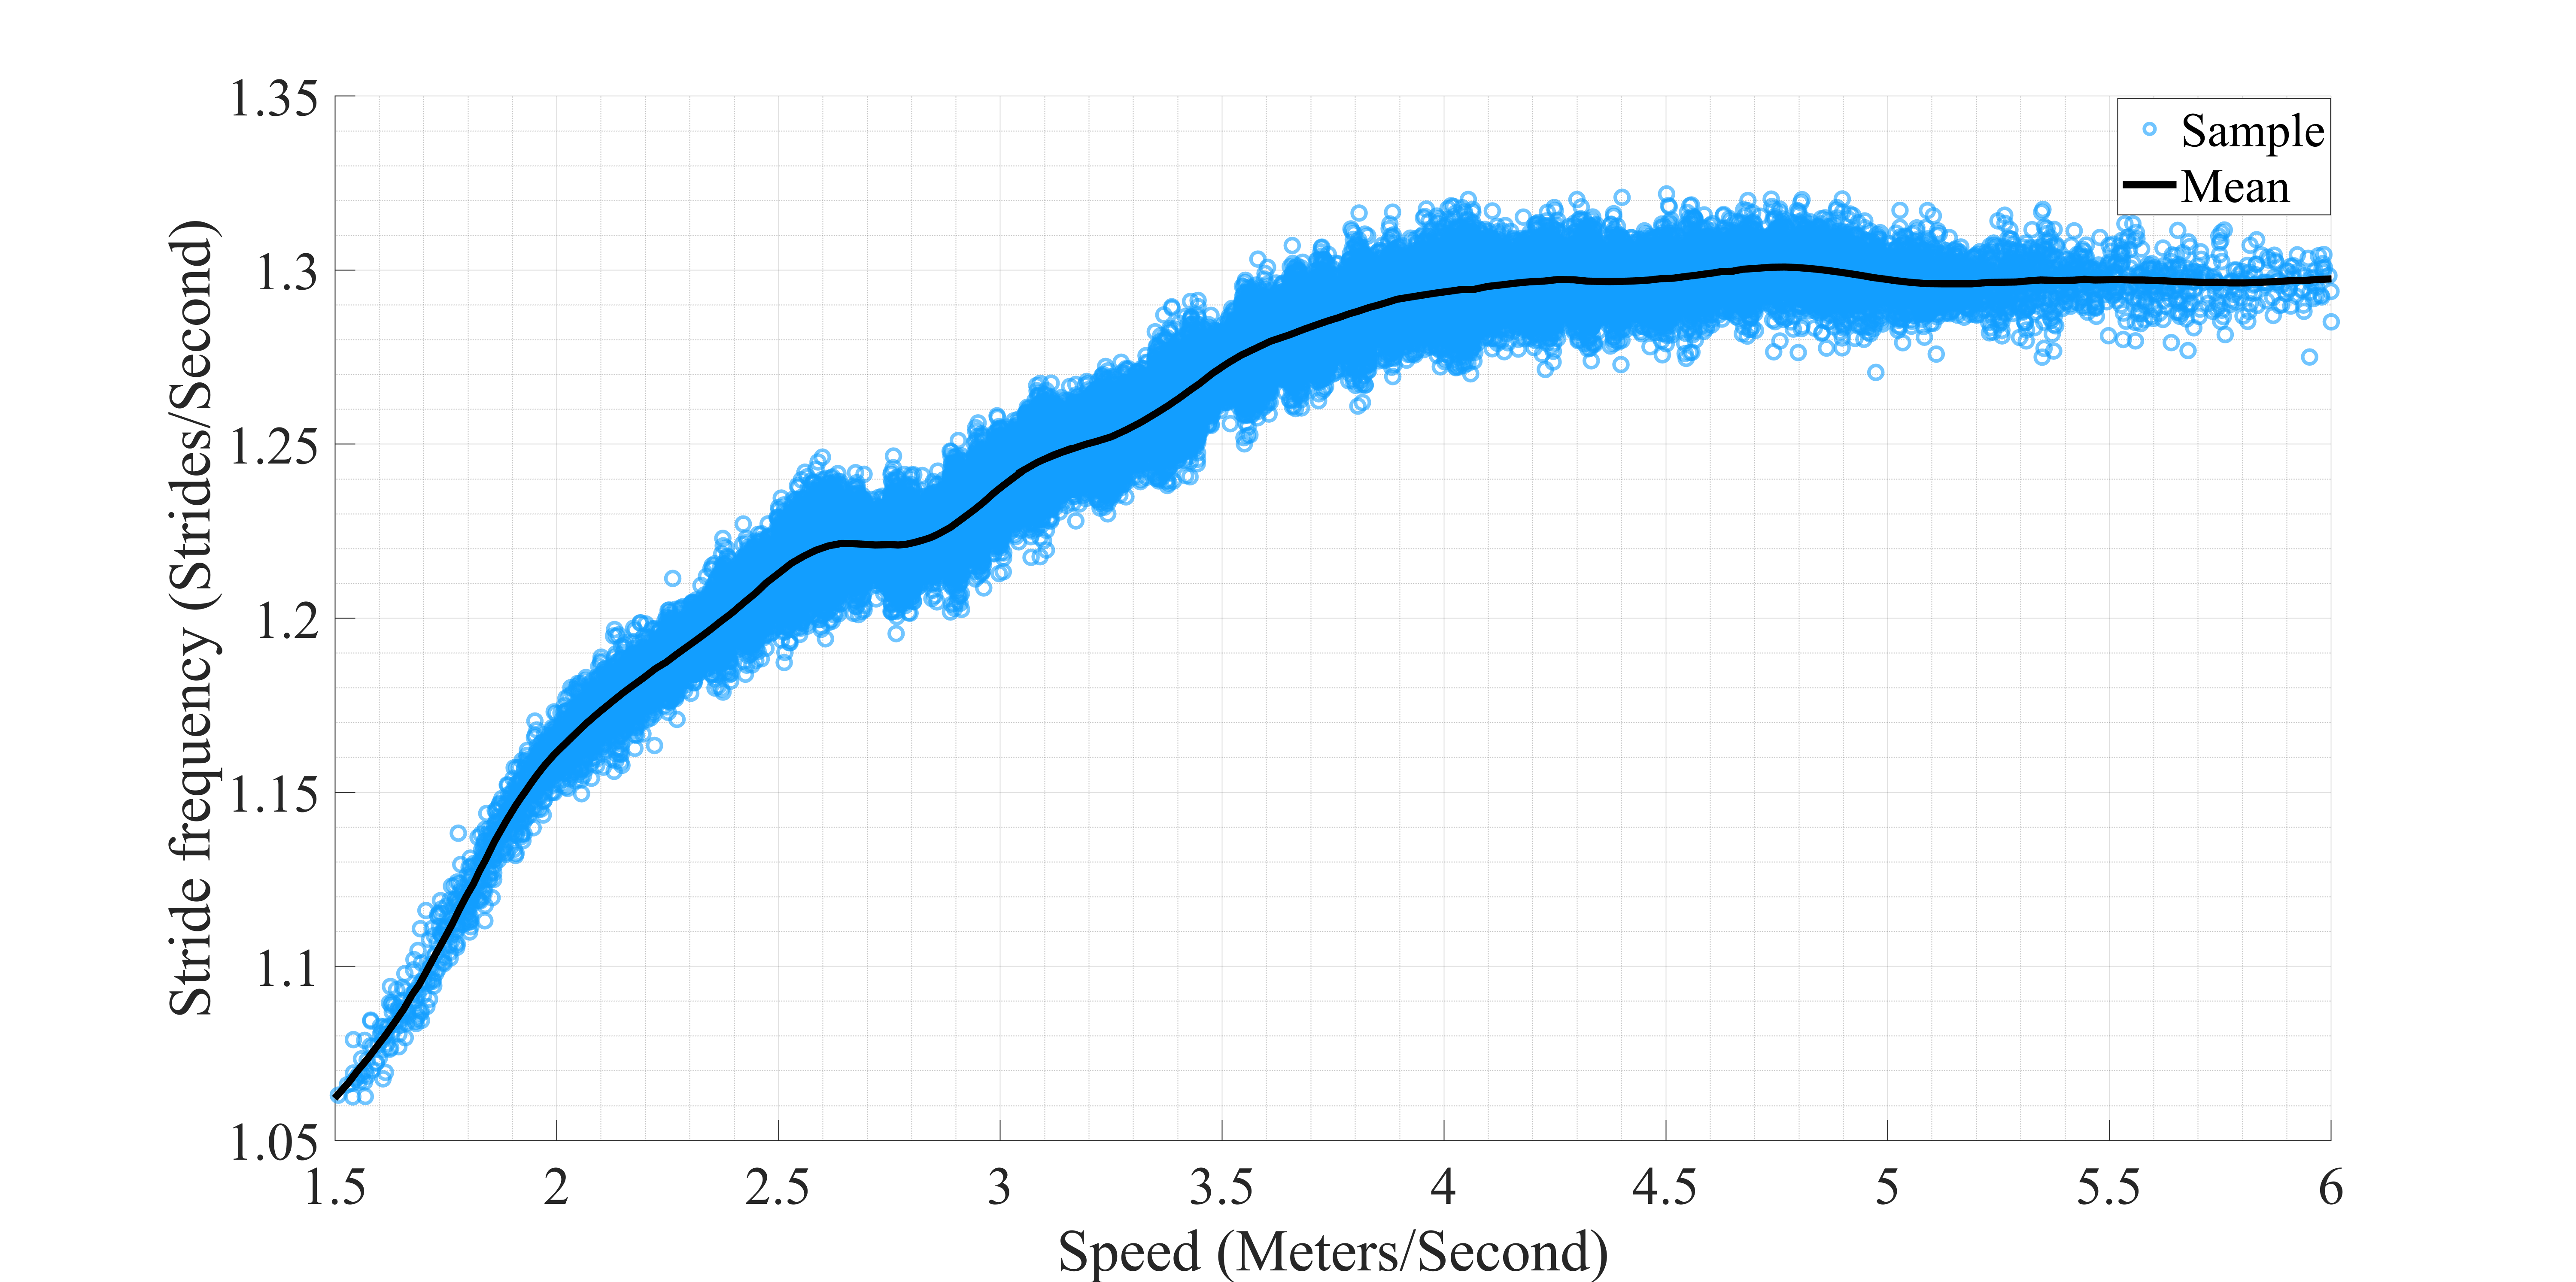
\includegraphics[width=\linewidth]{chapters/Speed/figures/untitledd_HQ.png}
\caption{Stride frequency versus speed.}
\label{stridevsspeed}
\end{figure}

The performance of all the models per gait had a similar pattern in the means of \gls{rmse} and normalized \gls{rmse}. To present this pattern, the performance of the model based on All feature set was demonstrated in Table \ref{resultsperrgait}. As the horses switched to faster gaits- from walking to cantering- the \gls{rmse} of models increased while their normalized \gls{rmse} slightly decreased. It should be noted that \gls{rmse} indicates the actual differences from the mean while normalized \gls{rmse} shows the differences relative to mean. Therefore, these alteration suggests that the model maintains its high accuracy on different speeds regardless of the gait.

random forest, \gls{gpr}, and \gls{svm} models obtained better results compared to decision tree and \gls{gbt}. Moreover, the performance of models trained with random forest algorithms was the best and the training and testing duration were significantly shorter compared to the models based on \gls{svm} and \gls{gpr}. Therefore, this method not only has an advantage in accuracy but also reduces computational time.

Models based on wider windows (256 timesteps) performed slightly better than models based on narrower windows (128 timesteps). Horses stride duration during walk and trot can be higher than 0.64 seconds (128 timesteps). Some features, such as \gls{fft} coefficients, generate a useful value when extracted from at least a full stride. Therefore, it reflects its effect as higher error in the models based on 128 timesteps windows.
 
The model in this study is more accurate than the only other speed estimation model in equine literature (average \gls{rmse} = 0.43 m/s) \cite{Schmutz2020}. Moreover, our model is able to estimate the speed of two distinct breeds and five gaits by attaching an IMU to one of the seven body locations in contrast to the mentioned model, which estimates the speed of one breed during canter by attaching an IMU to the saddle. In addition, five machine learning techniques were compared for choosing the best performing while only \gls{svm} was used in \cite{Schmutz2020}. Therefore, our model is the most complete in terms of accuracy, IMU placement options, and different motion patterns (breed and gait) support in the equine literature.

Despite the scarcity of speed estimation studies in equine literature, various studies investigated human speed estimation using \gls{imu}. For instance, linear regression was applied to the output of a single IMU to estimate older adults' walking speed, where the model yielded \gls{rmse} $\approx$ 0.069 m/s accuracy \cite{Byun2019}. Another study also developed a walking speed estimation model using GPR, which achieved an accuracy (\gls{rmse}) of 0.066--0.095 m/s \cite{Zihajehzadeh2016}. By comparing the results of the present model and the mentioned studies, we can conclude that our model is more general than the models from human studies in terms of multiple motion patterns support and different IMU placements, while others focused only on estimating the walking speed \cite{Diez2018}. As shown in Table \ref{resultsperrgait}, the normalized \gls{rmse} range of the model was 4.12--11.76\%. By calculating the normalized \gls{rmse} range of \cite{Zihajehzadeh2016} (5.4--10\%) and \cite{Byun2019} (6.6--14.7\%), it can be derived that the model in this study can estimate the speed more accurately than aforementioned studies.

The high accuracy results in Table \ref{imumocap_table} indicates the robustness of the model to data from new horses owing to the leave one out cross validation approach during the training. Despite the fact that \gls{omc} is the gold standard for calculating the speed, it was not used as for training the models. There were two reasons for this decision. First, the size of dataset with \gls{gps} data was more than 36 times larger than the dataset with \gls{omc} and the latter was not adequate enough for training machine learning models. Second, the dataset with \gls{omc} was limited in terms of gait types and only consisted of walk and trot. Therefore, owing to the large dataset of GPS measurement, GPS was validated for speed measurement and then used as the label for training the regression model.

It is more attractive to predict the speed with only one sensor since it is cheaper and the deployment on a subject's body is simpler. However, according to the results, the model based on Sacrum/Right front limb feature set showed better accuracy than models based on single \gls{imu}. During the training and competition, the sacrum \gls{imu} may fall off, since it is attached to the horse with double-sided tape without a strap. Therefore, it might limit the usability of the sacrum-based models to research purposes. In contrast, the limbs \gls{imu}s can be fixed around the tendon boots. Finally, the accuracy differences between the Sacrum/Right front limb-based model and individual limb-based models (especially hind limbs) are negligible. Considering the easier deployment, using only one limb \gls{imu} for estimation is nearly as accurate while being more applicable during training and competitions.


